\clearpage
\section{Structuring scientific work - Workflow management}
\label{sec:workflows}
The process from data generation to a scientific publication can be usually split into individual steps performing only a subset of the complete processing requirend. The separation of these steps can occur on different levels from very coarse like the separation of the experiment and analysis to very fine where each individual processing step is implemented in a independent script.

Workflow management is a concept to organize the individual steps forming a process. The granularity of the steps to manage highly depend on the complexity of the tasks and the diversity of the processing steps. A common and generic example forming a workflow management system is a queueing system used for cluster computing. Here users submit a number of in the simplest case independent jobs (computing steps) which are then depending on the available resources scheduled and distributed to suitable compute resources. This is a simple example, because the individual processing steps typically do not depend on each other and only the required amount of resources and time needs to be taken into account when organizing the execution.

For scientific projects like the Reach-to-Grasp experiment described in \cref{sec:data} there are dependencies between individual steps of the process from data acquisition to publication (see \cref{fig:scidata_metadata_pipeline,fig:scidata_reachgraspio_diagram}). The workflow management concept has been applied in a number of scientifics fields like genomics or imaging data. In these fields a systematic approach to data processing and analysis is required and feasable, since the they are dealing with large and numerous datasets which exceed manual monitoring or processing power \citep[e.g.][]{Palm_2010}.
For these disciplines, there are a number of platforms and tools available to implement pre \& postprocessing as well as analysis processing steps: Galaxy\footnote{Galaxy, \url{https://galaxyproject.org}, RRID:SCR\_006281} an  open, web-based platform providing bioinformatics tools and services for data intensive genomic research, vistrails\footnote{VisTrails, \url{https://www.vistrails.org}, RRID:SCR\_006261} an open-source scientific workflow and provenance management system that provides support for simulations, data exploration and visualization, Taverna\footnote{Taverna, \url{https://taverna.incubator.apache.org}, RRID:SCR\_004437} a scalable, open source \& domain independent tools for designing and executing workflows,  GenePattern\footnote{GenePattern, \url{http://www.broadinstitute.org/cancer/software/genepattern}, RRID:SCR\_003201} a genomic analysis platform that provides access to hundreds of tools for gene expression analysis, proteomics, SNP analysis, flow cytometry, RNA-seq analysis, and common data processing tasks, Renku\footnote{Renku, \url{https://datascience.ch/renku}} an online software platform for reproducible and collaborative data science including workflow management aspects, Terra\footnote{\url{https://terra.bio/}} a scalable platform  for biomedical research for data analysis and collaboration, Ugene \cite{Okonechnikov_2012} a multiplatform open-source software for molecular biology and snakemake\footnote{Snakemake, url{https://snakemake.readthedocs.io/en/stable/}, RRID:SCR\_003475} a Python based language and execution environment for make-like workflows.

In this section we present the usage of snakemake as a workflow management tool as it is domain independent, slim and easily integrates with Python based projects, e.g. to the Reach-to-Grasp and related projects \cref{sec:data}.

\subsection{Workflow management tools - Snakemake}
\label{sec:snakemake}
Snakemake is a generic workflow management tool derived from the build automation tool Make combined with Python features. It is available as bioconda\footnote{\url{https://anaconda.org/bioconda/snakemake}} and PyPi package\footnote{\url{https://pypi.org/project/snakemake}} with the latest version $5.5.4$ being considered here.

We demonstrate the basic features of snakemake based on two minimal workflow examples. The first one (\cref{code:workflows_simple_snakefile}) generates and copies files in two alternative ways and the second, more complex workflow uses two python scripts (\ref{code:workflows_python_scripts}) to generate data using \software{Neo} and visualize it using \software{Matplotlib} (\cref{code:workflows_python_snakefile,fig:python_demo}).

The description of individual steps of a workflow within snakemake is closely related to Make: A processing step is defined via its input and output files (\cref{code:workflows_simple_snakefile} line 11 and 12). The core of a rule is the instruction how to generate the output files based on the input files. Here snakemake offers multiple options based on direct execution of Python scripts or bash scripting. Bash scripts offer the most flexibility and are maked with the \code{shell} keyword (\cref{code:workflows_simple_snakefile} line 13). Within executed shell command references to the input and output files can be used via Python based reformatting of the command before execution. E.g. in \cref{code:workflows_simple_snakefile} line 13 the filename specified by the input of the rule \code{simple\_copy\_rule} (line 11) is automatically copied to the filename specified by the output of the rule by using \code{\{input\}} and \code{\{output\}} in the shell command. The same concept can be used to formulate snakemake rules in a more flexible fashion. E.g. in \cref{code:workflows_simple_snakefile} a set of flexible rules is introduces, which use an additional wildcard \code{\{filename\}} to be able to generate and copy not only files with filename \code{'file.md'}, but any markdown file. Here, the value of the variable \code{\{filename\}} is only determined during the exectution of the workflow. Therefore the same rule can be used multiple times within a workflow with different wildcard parameters. Hereby the value of the wildcard is determined recursively by the required output file.

The dependencies between snakemake rules are evaluated based on required files. By default snakemake uses the first rule within a \code{Snakefile} as main rule and tries to execute this rule. Alternatively snakemake can be called with an filename as an argument. In this case snakemake attempts to build the requested file based on all available rules matching in and output files of rules and checking the availability of basic input files. For this purpose snakemake generates an acyclic directed graph of rule dependencies (e.g. see \cref{fig:workflows_python_snakefile}) and infers all wildcard parameters from this. In case multiple rules can be used for generation of the same file a rule priority order can be be defined (\cref{code:workflows_simple_snakefile} line 1-3). Snakemake only executes rules and creates or overwrites files if the output files of a rule does not exist or the input files have a more recent modification time stamp the output files. This guarantees, that the output files of a snakemake workflow are always based on the most recent version of input files and at the same time minimizes the computational overhead, since only required or outdated files are generated.

Snakemake rule can be executed in dedicated containerized environments. For Python workflows snakemake supports the build of conda environments on a rule level. For each rule the conda environment can be defined via a \code{yaml} files specifying the required dependencies (see \cref{code:workflows_python_snakefile} snakefile line 16 and 23 and environments). Snakemake builds the environment using conda when requiring it the first time and keeps a reference. In case the \code{yaml} environment definition changes, the environment is automatically regenerated.

\cref{code:workflows_python_snakefile} demonstrates a more complex workflow using generic Python scripts for data generating based no the \software{Neo} package and visualization using the Python \software{Matplotlib} package (\cref{code:workflows_python_scripts}. These scripts are implemented to be used as standalone scripts, executed and provided with arguments from the command line. Additionally, they are not relying on a fixed data format, but support any format available in the \software{Neo} framework. This, in combination with the explicit definition of the required python packages in form of \code{yaml} files make the scripts highly flexible and generic, such that they can be easily reused in different contexts and projects. Furthermore, the snakemake implementation of the workflow keeps the genericity of the code by providing flexibility in the used data format, which is defined via an additional configuration \code{yaml} file, and the usage of the usage of wildcards for flexible handling of filenames. The resulting snakemake workflow as well as the output visualization of the randomly generated data can be seen in \cref{fig:python_demo}.


\begin{codeenv}
\textbf{Snakemake header}
\inputminted[firstline=1, lastline=3, linenos,tabsize=2,breaklines, fontsize=\scriptsize]{bash}{figures/workflows/simple_demo.snakefile}
\begin{multicols}{2}
\textbf{Simple rules}
\inputminted[firstline=5, lastline=13, linenos,tabsize=2,breaklines, fontsize=\scriptsize]{bash}{figures/workflows/simple_demo.snakefile}
\columnbreak
\textbf{Flexible rules}
\inputminted[firstline=15, lastline=23, linenos,tabsize=2,breaklines, fontsize=\scriptsize]{bash}{figures/workflows/simple_demo.snakefile}
\end{multicols}
\caption[Minimal snakemake example workflow]{Minimal snakemake example workflow. The workflow consists of two rules, for generation of a markdown file (.md) and conversion to a text file by plain copy of the content into a file with .txt extension. There are two versions of each rule demonstrating snakemake features at different complexities: The simple version of the rule handles filenames explicitely, whereas the flexible version of the rule is using wildcards to handle filenames. To resolve ambiguities between the two versions of the rules, we define a rule priority order in the first lines of the snakemake file.}
\label[codelisting]{code:workflows_simple_snakefile}
\end{codeenv}


\begin{codeenv}
\begin{multicols}{2}
\textbf{Snakefile}\\
\inputminted[firstline=1, lastline=40, linenos,tabsize=2,breaklines, fontsize=\scriptsize]{bash}{figures/workflows/python_demo.snakefile}
\columnbreak
\textbf{Environments}\\
\textbf{plotting\_environment.yaml}
\inputminted[linenos,tabsize=2,breaklines, fontsize=\scriptsize]{yaml}{figures/workflows/envs/plotting_environment.yaml}
\textbf{data\_generation\_environment.yaml}
\inputminted[linenos,tabsize=2,breaklines, fontsize=\scriptsize]{yaml}{figures/workflows/envs/data_generation_environment.yaml}
\textbf{config.yaml}
\inputminted[linenos,tabsize=2,breaklines, fontsize=\scriptsize]{yaml}{figures/workflows/config.yaml}
\end{multicols}
\caption[Snakemake example workflow for data generation and plotting]{Snakemake example workflow for data generation and plotting. The workflow consists of three rules, for data generation, data visualization and specification of the all output files of the workflow. The first two rules can be executed in dedicated conda environments, specified via the \code{conda:} directive and shown at the right. The workflow uses a configuration file (Snakefile line 1, \code{config.yaml}), specifying the format for storing \software{Neo} structures. This specification is also used to provide a constraint for wildcards with the name \code{data\_ext}, which resolves ambiguities between the data generation and visualization rule. The rule \code{all}, is by default executed when snakemake is run, it specifies two required output formats of the workflow. For the visualizaion of the workflow diagram when running the \code{all} rule see \ref{fig:python_demo}.}
\label[codelisting]{code:workflows_python_snakefile}
\end{codeenv}

\begin{figure}
%     \begin{multicols}{2}
    \begin{minipage}[t]{0.4\textwidth}
    \textbf{A}\\
    \includesvg[width=\textwidth, pretex=\relscale{0.8}]{figures/workflows/python_demo_escus}
    \end{minipage}
    \begin{minipage}[t]{0.6\textwidth}
%     \columnbreak\\
    \textbf{B}\\
    \includesvg[width=\textwidth]{figures/workflows/data}\\
    \end{minipage}
    %     \end{multicols}
 \caption[Snakemake example workflow for data generation and plotting]{Snakemake example workflow for data generation and plotting. The workflow diagram (left) and result (right). The workflow consists of two rules of which the \code{plot\_data} rule is executed twice with different parameters to generate the final plot in two file formats (\code{ext: svg}, \code{ex:png}, respecively). Different rules are color coded and the rule name is indicated at the top of each node. The frame style (solid/dashed) indicates if this rule needs to be run to generate a final output file. The arrows indicate the dependencies between the rule executions, rules at the top need to be executed first, since they generate output files that are required as input for the subsequent rules executions.}
\label{fig:python_demo}
\end{figure}


\begin{codeenv}
\begin{multicols}{2}
\textbf{Data generation}
\inputminted[linenos,tabsize=2,breaklines, fontsize=\scriptsize]{python}{figures/workflows/generate_data.py}
\columnbreak
\textbf{Data visualization}
\inputminted[linenos,tabsize=2,breaklines, fontsize=\scriptsize]{python}{figures/workflows/plot_data.py}
\end{multicols}
\caption[Standalone Python scripts used in \cref{code:workflows_python_snakefile}]{Standalone Python scripts used in \cref{code:workflows_python_snakefile}. The two scripts for data generation and visualization contain generic functions, relying on command line parameters to provide the arguments for the function calls (line 21-24 and line 18-21, respectively). The \textbf{data generation} is split into two functions, one for generation of the \software{Neo} structure (\code{generate\_neo\_data}) and one for saving the \software{Neo} structure to disc (\code{save\_neo\_block}). The first function generates a \software{Neo} \code{Block} containing a single \code{AnalogSignal} with randomly generated data (line 4-12). The second function recieves an generic \software{Neo} \code{Block} and saves it in the format specified by the provided filename (line 16-19). If the script is executed from the command line the input parameter \code{filename} is extracted from the command line arguments and both functions are executed consecutively, passing the \software{Neo} \code{Block} from one function the next (line 21-24). The \textbf{data visualization} uses the same concept as the data generation. Here the two internal functions are loading a \software{Neo} block from the specified data source filename (\code{load\_neo\_block}, line 4-7) and visualize the first \code{AnalogSignal} of a given plot, saving the result in a requested filename (code{plot\_analogsignal}, line 9-16). Both functions are called if the script is called from the command line and the two parameters specifying the data location as well as the output plot filename are extracted from the command line arguments.
}
\label[codelisting]{code:workflows_python_scripts}
\end{codeenv}

In addition to the features demonstrated in the example scripts, snakemake integrates well distributed storage concepts, such as Google Cloud Storage\footnote{Google Cloud Storage\url{https://cloud.google.com/storage/}}, DropBox\footnote{DropBox\url{https://www.dropbox.com}} or the secure shell protocol (SSH). Remote file sources are declared in the header of the snakemake file and individual files can be referenced from these sources in the same manner as local files. Besides access to remote files, snakemake also integrates with high-performance compute clusters by supporting common queueing systems such as the slurm workload manager\footnote{slurm, \url{https://slurm.schedmd.com}}. Here, a configuration file can be used to specify the custer job parameters on a rule-level, permitting detailed resource management.

\paragraph{Summary}
We presented the application of basice snakemake workflow features based on two example workflows demonstrating the modularization of a workflow into individual rules and their file-based dependency handling. We highlighted the flexibility of this approach by introducing wildcard based filename handling and explained the snakemake dependency graph. We provide examples of generic standalone Python scripts for seamless integration into snakemake rules and demonstrated advanced configuration features of the workflow via additional configuration files and wildcard constraints. We introduce additional features for integration of remote files and cluster usage.
The presented features make snakemake our tool of choice for the implementation of scientific workflows, as it provides a domain-independent and slim option for workflow definition which integrates well with existing scripted data processing steps.


\todo{inspiration from computer sciences \& industrial software development: Continuous integration \& deployment}



\subsection{Practical application}
Snakemake has been applied in a variety of different fields and projects. Many of the provided examples and tutorials are set in the field of genomics\footnote{\url{https://snakemake.readthedocs.io/en/stable/getting_started/examples.html}}\footnote{\url{https://snakemake.readthedocs.io/en/stable/tutorial/basics.html}} here we present a workflow design in the context of the Vision4Action project, a successor project of Reach-to-Grasp.

\subsubsection{The Vision-For-Action project}
The Vision-For-Action project is building on top of the Reach-to-Grasp project by extending the investigation of motor control only to the interaction of motor and visual activity. For this a modified task is used, involving the continuous integration of visual input and motor control. The experimental hardware is a Real-time visuomotor behavior and electrophysiology recording
(RIVER) setup and consists partially of the same components used in the Reach-to-Grasp experiment. For a detailed description of the recording setup see \cite{deHaan_2018,deHaan_2018a}. The Reach-to-Grasp experiment was extended by an eye as well as hand movement control system and a complex task design including the sequential pointing to up to six targets. To the current date, only a single monkey was recorded in the Vision-For-Action setup.

\paragraph{The task}
In the context of the Vision-For-Action experiment the monkey views a horizontal, semi-transparent mirror on which a red dot is projected corresponding to the location of the monkeys hand below the mirror (\cref{fig:river_setup}). The monkey is trained to initialize a task by moving the hand curser into the area of a central, illuminated target. After a waiting period the central target is deactivated and depending on the task type one or multiple of 6 peripheral targets are illuminated. The to recieve a reward, the monkey has to deactivate all illuminated targets by moving the hand curser into the target. Depending on the task also additional targets might be activated when deactivating the previous target. Two classic task types are implemented currently: The the landing task, in which the monkey is presented a sequence of three peripheral targets, which he has to deactivate by staying in the targets for $100ms$ leading to direct movements to the target. The drawing task, in which the monkey is presented multiple targets at once and can chose an order and route to deactivate these. In this task type the monkey only briefly needs to touch the target with the hand curser leading to very curved movement trajectories. 
\todo{is this already published somewhere? am I permitted to write this?}


\paragraph{The setup}
The RIVER setup consists of four components, which integrates three subsetups covering different modalities. The three components are the recording of the neural activity via a \software{Blackrock} system described in the context of the Reach-to-Grasp experiment, the tracking of eye movement via a an EyeLink system and the tracking / control of the arm movement via a Kinarm motorized exoskeleton of the arm (\cref{fig:river_setup}).

As in the Reach-to-Grasp experiment, neural activity is recorded using Utah array technology. However, instead of a single Utah array implanted in motor cortex, in the Vision-for-Action experiment, an additional Utah array split into $4$ smaller arrays is implanted in visual cortical array. Each Utah array part consists of $6\times6$ electrodes, resulting in a total of $96$ active recording electrodes in motor cortical area M1 and premotor cortex and $32$  active electrodes in vision-related cortical areas V1, V2, 7a and DP. The two Utah arrays are recorded using two recording setups in parallel (see \cref{fig:river_setup} purple panels). This includes two separate connectors implanted contralateral to the Utah arrays, ipsilateral to the active hand of the monkey. The two connectors are during a recording session each connected to a separate headstage including a neural signal amplifier, digitizer and converter. The signals are then optically transmitted to a real-time Neural Signal Processor (NSP) which performs online signal processing (filtering, spike extraction and sorting). In the next step, the processed neuronal signals of each NSP are transmitted to a corresponding offline Cerebus computer for writing to disc and monitoring by the experimenter.

The active arm of the monkey is attached to a Kinarm system, which can be used to track and interfer with the monkey's movement (\cref{fig:river_setup} green panels). The kinarm restricts the hand movement to a horizontal plane below the working space of the monkey and can be used to exert forces onto the monkey's arm. Online feedback of the hand location is provided visually in form of a circular red curser in the working space.

The gaze position of the monkey is tracked using an EyeLink system (\cref{fig:river_setup} blue panels). To be able to record the gaze position, the monkeys head is placed in a plastic head mask, restricting large head movements and providing acces to the reward system. The gaze direction is infered from a video signal showing the cornea reflection of an infrared light source. The raw eye direction signal is online processed using the kinarm real-time system to arrive at the final eye position signal. This conversion depends on the exact location of the monkey's eye with respect to the camera and light source and therefore needs to be calibrated frequently to ensure a stable gaze position recording. For a detailed description of the configuration mechanism and procedure, see \citet{deHaan_2018}.

All online tracked signals, neuronal, kinarm as well as gaze are input to at least one of the  two NSPs, resulting in two sets of \software{Blackrock} files as original data files generated by the RIVER setup.

The experiment control is implemented in a Simulink model on the kinarm realtime computer. This model coordinates the experiment using a Stateflow description of the experimental task and generating corresponding event signals encoding the state of the system. The event codes are unique and globally defined in a generic manner by encoding events using a $16$ bit code. Of the $65536$ possible codes, $1246$ codes are mapped to generic experimental events like a trial start or the beginning of a trial metadata sequence. This leaves $64290$ unused codes, providing sufficient flexibility for future extensions of the schema. For robustness, all event codes come in pairs of two, embracing the metadata information in a start and end bracket. The globally defined experimental codes follow a systematic schema grouping events based on their first digit in six categories: 'Experiment Metadata', 'Trial Metadata', 'Screen Related', 'Exoskeleton Related', 'Other', 'Behaviour Related' and 'Error'. For more details on the global encoding of metadata see \citet{deHaan_2018a}.
For a specific task implementation used in the experiment, a mapping of the globally defined codes to the task specific metadata was defined. This approach permits the global use of generic event codes in the recorded data which at the same time is capable of capturing all task specific metadata. The global event codes generated by the Simulink model are together with hand and gaze location information forwarded to the Blackrock system and saved together with the neuronal signals.

\paragraph{Synchronization}
For coherent data recording from three different systems a shared time frame between all of them is essential for the interpretation of the data. The RIVER setup produces two sets of \software{Blackrock} files since all other signals are integrated online during the recording. The two NSPs provide a synchronization feature, permitting the synchronization of the two systems upon start up of the recording system. To ensure continuous synchrony between the two systems the two NSPs recieve common input from the kinarm system, which can be offline used for validating the common recording time frame.

\paragraph{Data and metadata files}
The RIVER setup generates two sets of \software{Blackrock} recording data files: one containing neural signals from motor and the other from visual cortical areas in the \code{ns6} format. In addition both datasets contain partially identical behavioral signals for the hand, arm and gaze position in the \code{ns2} format(\cref{tab:v4a_recording_files}). In addition also the position of the active target is stored with a $1kHz$ sampling rate as well as the synchronization signals which are shared between the two NSP / Cerebus systems.
Same as for the Reach-to-Grasp experiment, the \code{nev} file also contains online extracted spikes, but in addition it also captures a large amount of structured metadata in form of events, which encode experimental metadata in a generic fashion.
These metadata are complemented by a set of metadata descriptors. These are text files in \code{csv} format, structured in an \software{odMLtables} compatible fashion. These files generated by the experimenter in a manual, but strongly programming aided fashion. The content of these files contains a basic structure for metadata branches to be integrated in an hierarchical \software{odML} metadata collection. A complete set of descriptor files comprises $9$ \code{csv} files and covers all metadata not captured in the event recording file. Essential metadata stored in these \code{csv} files is information about the monkey, the hardware components used, the global and specific codes used in the session, the signal flow for digital and analog signals in the recording setups and the general description of the recording session and meta information about all required descriptor files (\ref{tab:v4a_metadata_files}). Additionally configuration and supplemental files that can not be captured in a csv file but are used during the recording are referenced in the session descriptor. Most of the metadata files are constant across sessions, some change with the task type and only a few need to be generated / tracked explicitely for each session. Nevertheless, we decided to copy even seemingly constant metadata files for each session anew, since during the life time of the experiment also some these metadata can change unexpectedly, e.g. when a part of the setup needs to be replaced due to malfunction.




\begin{sidewaysfigure}
 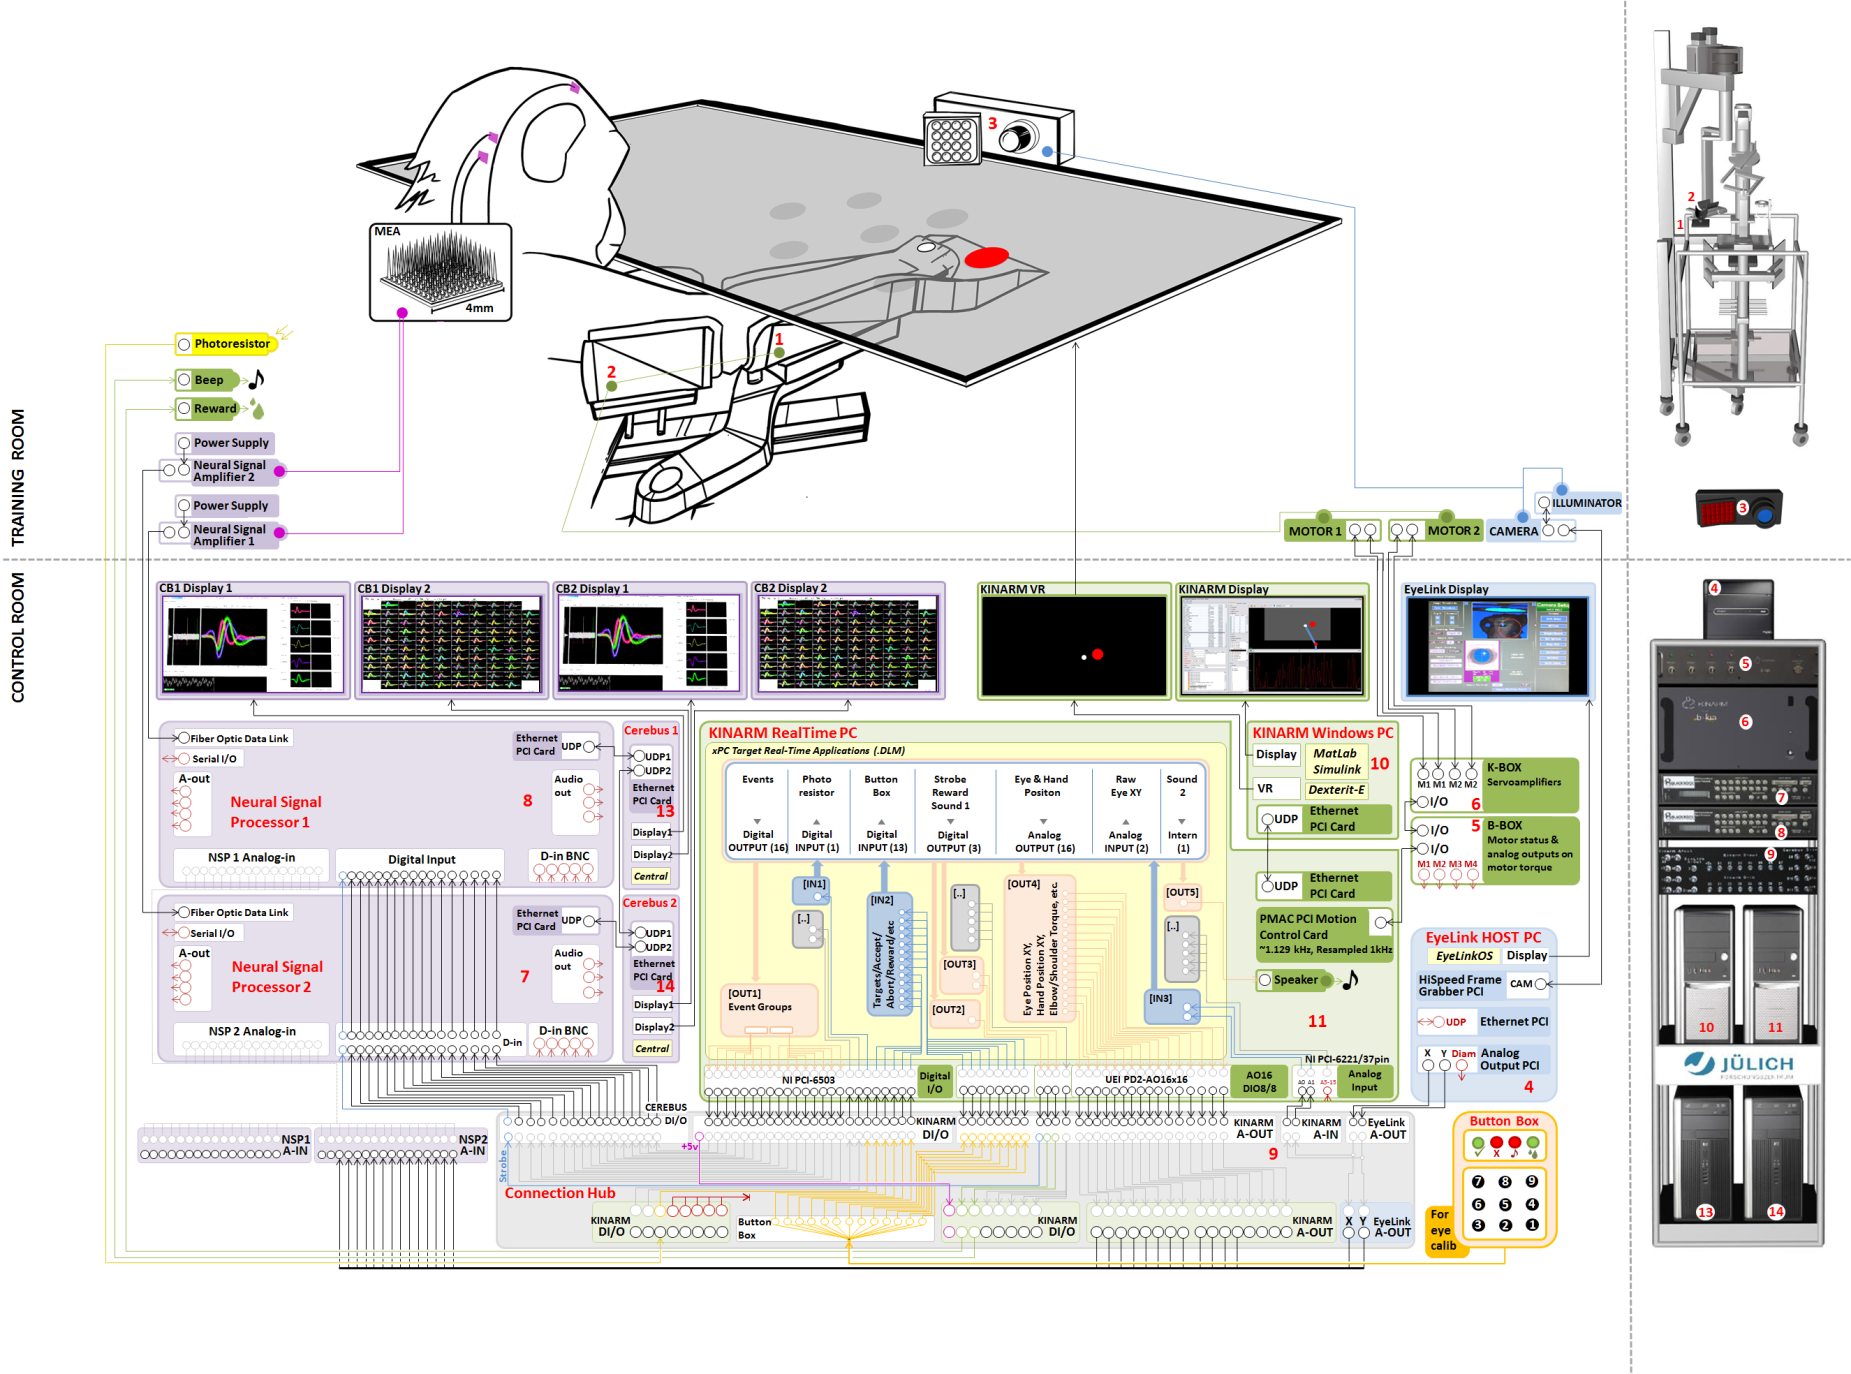
\includegraphics[width=0.8\textwidth]{figures/workflows/river_setup_hardware}
 \caption[The RIVER setup]{The RIVER setup including schematic of hardware components and signal flows. Depicted are the monkey task setup (top right), the recording system and signal flows (bottom left), the monkey chair and kinarm (top right) and the recording hardware rack (bottom right). Figure from \citet{deHaan_2018a}.}
 \label{fig:river_setup}
\end{sidewaysfigure}


\begin{table}[]
\begin{tabular}{|l|l|}
\hline
file format & content                                               \\ \hline
*.ccf       & cerebus configuration                                 \\ \hline
*.nev       & digital events                                        \\
            & \textbullet~ unsorted spiketimes                      \\
            & \textbullet~ spike waveforms                          \\
            & \textbullet~ experiment metadata                      \\
            & \textbullet~ trial metadata                           \\
            & \textbullet~ screen events                            \\
            & \textbullet~ exosceleton events                       \\
            & \textbullet~ behavioural events                       \\
            & \textbullet~ errors                                   \\
            & \textbullet~ ...                                      \\ \hline
*.ns2       & continous signals with $1kHz$ sampling rate           \\
            & \textbullet~ eye (gaze) position                      \\
            & \textbullet~ hand position                            \\
            & \textbullet~ target position                          \\
            & \textbullet~ elbow position                           \\
            & \textbullet~ joint angles / velocities / accelerations \\
            & \textbullet~ synchronization pulses                   \\ \hline
*.n6        & continous signals with $1kHz$ sampling rate           \\
            & \textbullet~ neuronal signals                         \\ \hline
\end{tabular}
\caption[Recording file formats and content in the Vision-for-Action project]{Recording file formats and content in the Vision-for-Action project. The cerebus configuration is saved in a custom \software{Blackrock} configuration format. The nev format contains digital events generated by the NSP based on the neuronal activity (spike detection) and all integrated events from additional hardware systems. Continuous signals are stored in different files depending on the sampling resoulution. At a low sampling resolution of $1kHz$ the ns2 signal contains behavioral signals whereas the neuronal high sampling resolution signals are stored in the ns6 file.}
\label{tab:v4a_recording_files}
\end{table}

\begin{table}[]
\scriptsize
\begin{tabular}{lll}
\textbf{Descriptor}                                & \textbf{Content}                                                                                                       & \textbf{Generation}                                                                  \\ \hline
\multicolumn{1}{|l|}{session}                      & \multicolumn{1}{l|}{\textbullet~ session name}                                                                         & \multicolumn{1}{l|}{once per session}                                                \\
\multicolumn{1}{|l|}{}                             & \multicolumn{1}{l|}{\textbullet~ relevant metadata files}                                                              & \multicolumn{1}{l|}{semi-automatic}                                                  \\
\multicolumn{1}{|l|}{}                             & \multicolumn{1}{l|}{\textbullet~ task type}                                                                            & \multicolumn{1}{l|}{visual cross check}                                              \\
\multicolumn{1}{|l|}{}                             & \multicolumn{1}{l|}{\textbullet~ ...}                                                                                  & \multicolumn{1}{l|}{}                                                                \\ \hline
\multicolumn{1}{|l|}{subject}                      & \multicolumn{1}{l|}{\textbullet~ species}                                                                              & \multicolumn{1}{l|}{onetime, static}                                                 \\
\multicolumn{1}{|l|}{}                             & \multicolumn{1}{l|}{\textbullet~ active hand}                                                                          & \multicolumn{1}{l|}{}                                                                \\
\multicolumn{1}{|l|}{}                             & \multicolumn{1}{l|}{\textbullet~ training}                                                                             & \multicolumn{1}{l|}{}                                                                \\
\multicolumn{1}{|l|}{}                             & \multicolumn{1}{l|}{\textbullet~...}                                                                                   & \multicolumn{1}{l|}{}                                                                \\ \hline
\multicolumn{1}{|l|}{kinarm}                       & \multicolumn{1}{l|}{\textbullet~ hardware specifications}                                                              & \multicolumn{1}{l|}{onetime, static}                                                 \\
\multicolumn{1}{|l|}{}                             & \multicolumn{1}{l|}{\textbullet~ programming software}                                                                 & \multicolumn{1}{l|}{}                                                                \\
\multicolumn{1}{|l|}{}                             & \multicolumn{1}{l|}{\textbullet~ ...}                                                                                  & \multicolumn{1}{l|}{}                                                                \\ \hline
\multicolumn{1}{|l|}{eyelink}                      & \multicolumn{1}{l|}{\textbullet~hardware specifications}                                                               & \multicolumn{1}{l|}{onetime, static}                                                 \\
\multicolumn{1}{|l|}{}                             & \multicolumn{1}{l|}{\textbullet~ software specifcations}                                                               & \multicolumn{1}{l|}{}                                                                \\
\multicolumn{1}{|l|}{}                             & \multicolumn{1}{l|}{\textbullet~ ...}                                                                                  & \multicolumn{1}{l|}{}                                                                \\ \hline
\multicolumn{1}{|l|}{blackrock}                    & \multicolumn{1}{l|}{\textbullet~ Utah arrays}                                                                          & \multicolumn{1}{l|}{onetime, static}                                                 \\
\multicolumn{1}{|l|}{}                             & \multicolumn{1}{l|}{\textbullet~ connectors}                                                                           & \multicolumn{1}{l|}{}                                                                \\
\multicolumn{1}{|l|}{}                             & \multicolumn{1}{l|}{\textbullet~ physical properties}                                                                  & \multicolumn{1}{l|}{}                                                                \\
\multicolumn{1}{|l|}{}                             & \multicolumn{1}{l|}{\textbullet~ ...}                                                                                  & \multicolumn{1}{l|}{}                                                                \\ \hline
\multicolumn{1}{|l|}{analog\_communication}        & \multicolumn{1}{l|}{\textbullet~ hardware specifications}                                                              & \multicolumn{1}{l|}{onetime, static}                                                 \\
\multicolumn{1}{|l|}{}                             & \multicolumn{1}{l|}{\textbullet~ pin mapping}                                                                          & \multicolumn{1}{l|}{}                                                                \\
\multicolumn{1}{|l|}{}                             & \multicolumn{1}{l|}{\textbullet~ ...}                                                                                  & \multicolumn{1}{l|}{}                                                                \\ \hline
\multicolumn{1}{|l|}{digital\_communication}       & \multicolumn{1}{l|}{\textbullet~ hardware specifications}                                                              & \multicolumn{1}{l|}{onetime, static}                                                 \\
\multicolumn{1}{|l|}{}                             & \multicolumn{1}{l|}{\textbullet~ pin mapping}                                                                          & \multicolumn{1}{l|}{}                                                                \\
\multicolumn{1}{|l|}{}                             & \multicolumn{1}{l|}{\textbullet~ ...}                                                                                  & \multicolumn{1}{l|}{}                                                                \\ \hline
\multicolumn{1}{|l|}{codes\_global}                & \multicolumn{1}{l|}{\textbullet~ code mapping \& definition}                                                           & \multicolumn{1}{l|}{onetime, static}                                                 \\ \hline
\multicolumn{1}{|l|}{codes\_task}                  & \multicolumn{1}{l|}{\textbullet~ mapping of global codes to}                                                           & \multicolumn{1}{l|}{once per task type}                                              \\
\multicolumn{1}{|l|}{}                             & \multicolumn{1}{l|}{\hspace{1cm} task specific metadata}                                                               & \multicolumn{1}{l|}{static}                                                          \\ \hline
\textbf{Additional metadata files}                 &                                                                                                                        &                                                                                      \\ \hline
\multicolumn{1}{|l|}{task description (pdf)}       & \multicolumn{1}{l|}{\begin{tabular}[c]{@{}l@{}}extensive human readable task description\\ with sketches\end{tabular}} & \multicolumn{1}{l|}{\begin{tabular}[c]{@{}l@{}}once per task,\\ static\end{tabular}} \\ \hline
\multicolumn{1}{|l|}{task model (mdl)}             & \multicolumn{1}{l|}{model description file as used by SimuLink}                                                        & \multicolumn{1}{l|}{\begin{tabular}[c]{@{}l@{}}once per task,\\ static\end{tabular}} \\ \hline
\multicolumn{1}{|l|}{task parameter file (dtp)}    & \multicolumn{1}{l|}{task parameter file as used by SimuLink}                                                           & \multicolumn{1}{l|}{\begin{tabular}[c]{@{}l@{}}once per task,\\ static\end{tabular}} \\ \hline
\multicolumn{1}{|l|}{target picture (png)}         & \multicolumn{1}{l|}{image used for visual targets}                                                                     & \multicolumn{1}{l|}{onetime}                                                         \\ \hline
\multicolumn{1}{|l|}{calibration parameters (mat)} & \multicolumn{1}{l|}{parameters of the calibration model}                                                               & \multicolumn{1}{l|}{onetime}                                                         \\ \hline
\multicolumn{1}{|l|}{calibration data (mat)}       & \multicolumn{1}{l|}{data used for calibration}                                                                         & \multicolumn{1}{l|}{once per calibration}                                            \\ \hline
\end{tabular}
\caption[Metadata files in the Vision-for-Action project]{Metadata descriptors and supplementary files in the Vision-for-Action project. Nine \code{csv} descriptor files are required for a complete description of the experiment. Most of these only need to be generated once as the contained data should be static. Only the session descriptor needs to be adjusted each session as well as the task code descriptor if a new task was introduced. There are six additional files which provide supplemental metadata information. These provide additional configuration and image material used during the recording.}
\label{tab:v4a_metadata_files}
\end{table}

\subsection{Metadata workflow in the Vision-for-Action project}

Based on the metadata source files described in \cref{tab:v4a_metadata_files} we designed a workflow for metadata collection and enrichment which consisting processing steps that can be classified into one of five processing categories (\cref{fig:v4a_metadata_workflow_dag}). We implement the workflow using snakemake in combination with python scripts, which are implemented in a standalone fashion as described in \cref{sec:snakemake} (\cref{code:workflows_python_scripts}). In the context of this workflow we term these standalone python scripts 'application' ('app'). Each app performs only a single, definite processing step based on as few input files as possible, to avoid unnessesary dependencies.



\begin{figure}
    \centering
    \includesvg[width=\textwidth, pretex=\relscale{0.7}]{./figures/workflows/rulegraph_colored_escus}
    \caption[Metadata workflow rules for Vision-for-Action experiment]{Metadata workflow rules for Vision4Action experiment. Visualized are only the general dependencies between rules irrespective of the input parameters and multiple executions during the run of the workflow. Metadata are aggregated, data are loaded and combined in multiple workflow steps.}
    \label{fig:v4a_metadata_workflow_dag}
\end{figure}

\begin{sidewaysfigure}
    \textbf{A}\\
    \includesvg[width=\textwidth, pretex=\relscale{0.05}]{./figures/workflows/v4a_dag_all_descriptors_mod_escus}\\
    \vspace{1cm}
    \textbf{B}\\
    \includesvg[width=\textwidth, pretex=\relscale{0.01}]{./figures/workflows/v4a_dag_all_apps_mod_escus}\\
    \caption[Metadata workflow examples from Vision4Action experiment]{Example metadata workflow steps in the Vision-for-Action project.}
    \label{fig:v4a_metadata_workflow_dag}
\end{sidewaysfigure}


advantages:
- apps can be tested e.g. via unittest framework
- snakemake workflow can run in 'incomplete' mode

discussion
- additional overhead via repetetive data loading \& saving

\todo{introduce the concept of workflow management, snakemake, Apps,  categories
- general apps
- experiment specific apps}


% \subsection{Waves project}
\subsection{Summary \& Guidelines}
